\documentclass[11pt,twoside]{article}
\usepackage{asp2010}
\usepackage{graphicx}
\resetcounters

\bibliographystyle{asp2010}

\markboth{A. Costa et Al.}{VisIVO}

\begin{document}

\title{VisIVO: A Web-Based, Workflow-Enabled Gateway for Astrophysical Visualization}
\author{Costa A.$^1$, Bandieramonte M.$^2$, Becciani U.$^1$, Krokos M.$^3$, Massimino P.$^1$, Petta C.$^2$, Pistagna C.$^1$, Riggi S.$^1$, Sciacca E.$^1$, Vitello F.$^1$}
\affil{$^1$INAF Astrophysical Observatory of Catania, Italy}
\affil{$^2$University of Catania, Italy}
\affil{$^3$University of Portsmouth, U.K.}

\begin{abstract}
We present a web-based and workflow-enabled framework called VisIVO Gateway that allows integration of large-scale multidimensional datasets together with applications for visualization and exploration on Distributed Computing Infrastructures (DCIs).
Our framework is implemented through a workflow-enabled portal wrapped around WS-PGRADE which is the grid User Support Environment (gUSE) portal.  We provide customized interfaces for creating, invoking, monitoring and also modifying scientific workflows. All technical complexities, e.g. related to visualization algorithms and DCI configurations, are conveniently hidden from view.
A number of workflows are enabled by default, e.g. implementing local or remote uploading and creation of scientific movies. Scientific movies are useful not only to scientists for presenting their research results, but also to museums and science centres for engaging visitors with complex scientific concepts.
Our gateway can be accessed via standard www interfaces but also through a newly developed iOS mobile application offering novel ways for sharing analysis and exploration experiences with large-scale datasets in collaborative environments.
\end{abstract}

\section{Introduction}
Nowadays science gateways allow an increasing number of scientists from different communities to access large-scale distributed data infrastructures (DDI) and distributed computing infrastructures (DCI) reducing the time needed to learn and exploit new computational technologies \citep{borkin2011visualization}. The aim of a science gateway is to provide a graphical interface for access to DDIs / DCIs that is not only technology-neutral but also fully customized to the application domain of end-users \citep{abt_1990}. Our portal has been developed by using gUSE, WS-PGRADE  \citep{kacsuk2011p}  and VisIVO \citep{becciani2010visivo} technologies. This gateway provides an environment for exploring large-scale datasets dynamically detecting and analysing their properties through 3D visualization tools. 

\begin{figure}
\begin{center}
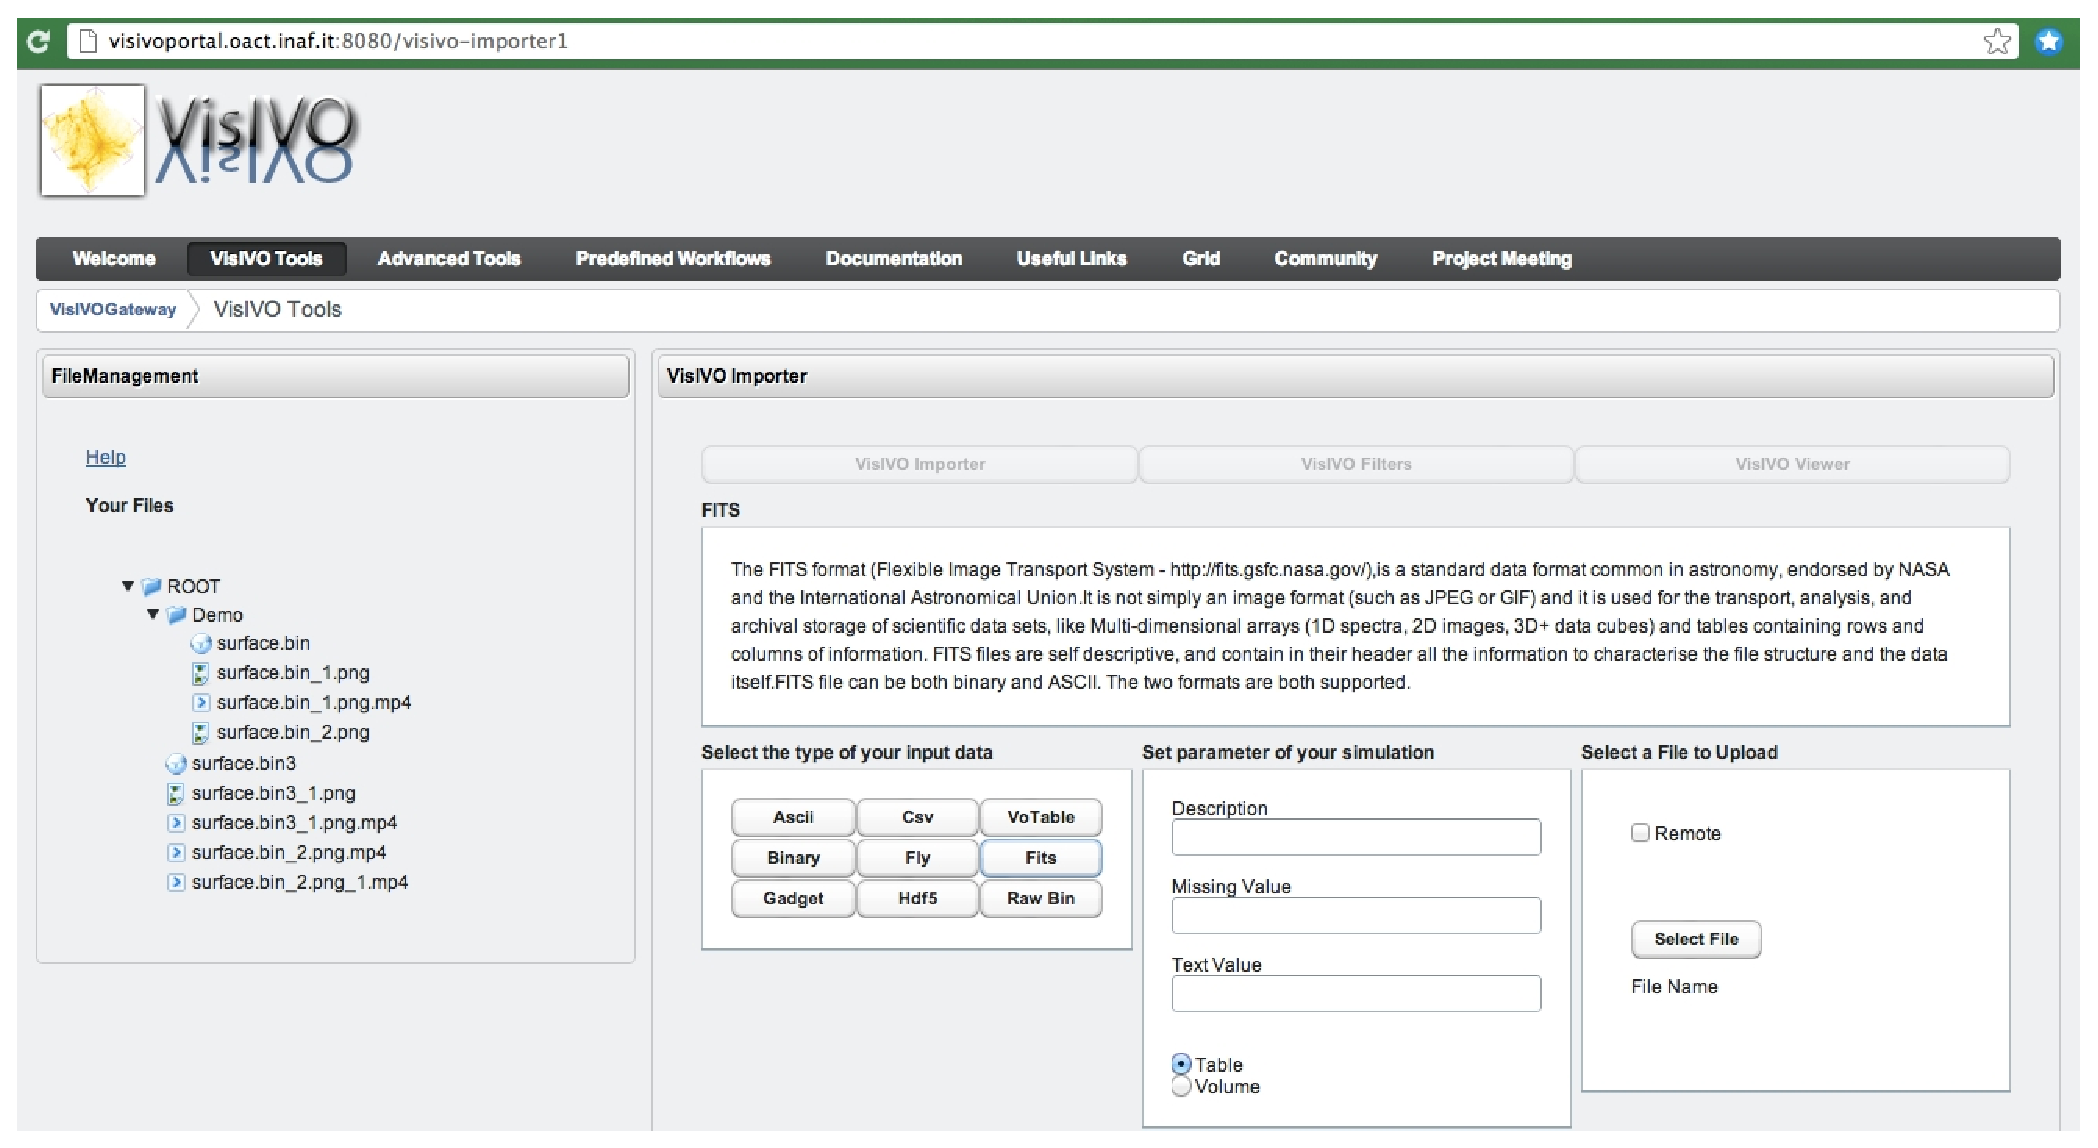
\includegraphics[width=1\textwidth]{O08_f1.eps} 
\caption{Data Management Facility (left) and FITS Importer (right).}\label{fg1}
\end{center}
\end{figure}

\section{Workflows and User Communities}
A VisIVO workflow is a directed acyclic graph where nodes represent \emph{jobs} (i.e. batch programs to be executed on computing elements),  \emph{ports} represent input and output files expected or produced by jobs and \emph{arcs} represent file transfer operations. The exploited WS-PGRADE technology offers not only nested but also recursive workflows, thus allowing application programmers to add control mechanisms to workflow graphs. Our science gateway supports astrophysical communities in two ways: either as advanced application developers who understand workflows and grid technology or as end-users who are not necessarily aware of such details. Our VisIVO science gateway allows application developers to access all advanced workflow features, such as creation of graphs, abstract workflows and templates. A built-in repository stores all workflow objects published by application developers to be downloaded and further developed by the community. End-users are not necessarily aware of underlying workflows and DCIs as the portal presents its functionality as a web toolkit of analysis and visualization tools. 

\begin{figure}
\begin{center}
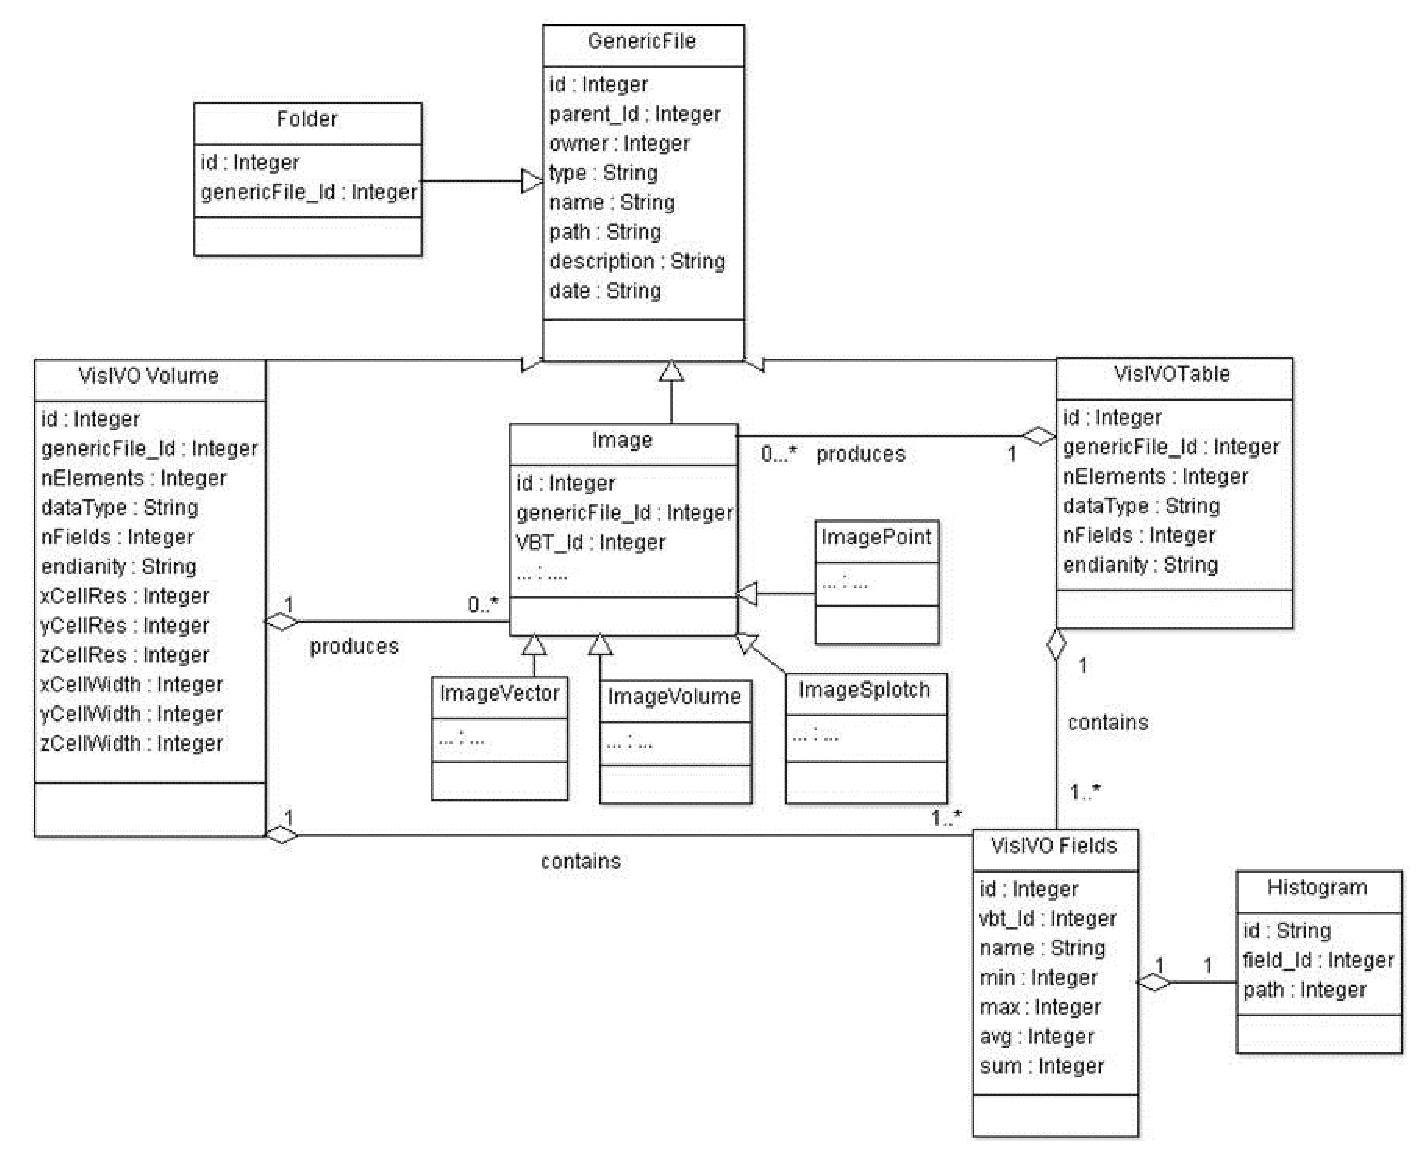
\includegraphics[width=0.7\textwidth]{O08_f2.eps}
\caption{Illustration of Data Base Schema Employed in VisIVO Science Gateway.}
\label{fg2}
\end{center}
\end{figure}

\section{Features and Services}
The authentication service employed is realised through OpenID, Facebook and local accounting. An interactive visualization service provides several knowledge discovery tools. These tools are constantly improved by incorporating novel algorithms for analysis and exploration of large-scale astrophysical datasets \citep{hassan2011scientific}. Visualization tools may allow for interactivity, e.g. by dynamically placing cameras or fine tuning of rendering parameters. Non interactive tools allow realizations of complex rendering tasks, e.g. movie creation.   

\section{Data Model}
The data-model determines the structure of user data allowing creation of a virtual file system. Images, datasets and movies are described by using a number of appropriate properties  and object relationships (see Figure \ref{fg1}). The GenericFile object contains attributes such as owner, creation time and location. The objects VisIVOTable and VisIVOVolume inherit from GenericFile and represent the basic types of files the portal deals with, i.e. tables and volume datasets. VisIVOTable defines attributes such as endianity, number of fields, data type and number of elements. VisIVOVolume defines attributes such as number and size of cells for each dimension. The VisIVOTable and VisIVOVolume objects produce several Image objects inheriting from the GenericFile and containing the VisIVOViewer parameter set, such as the image size, the camera position or color palette used. The portal provides a graphical interface (see Figure \ref{fg2}) for intuitive handling of user owned datasets, images and movies within a private staging area.

\begin{figure}
    \centering
    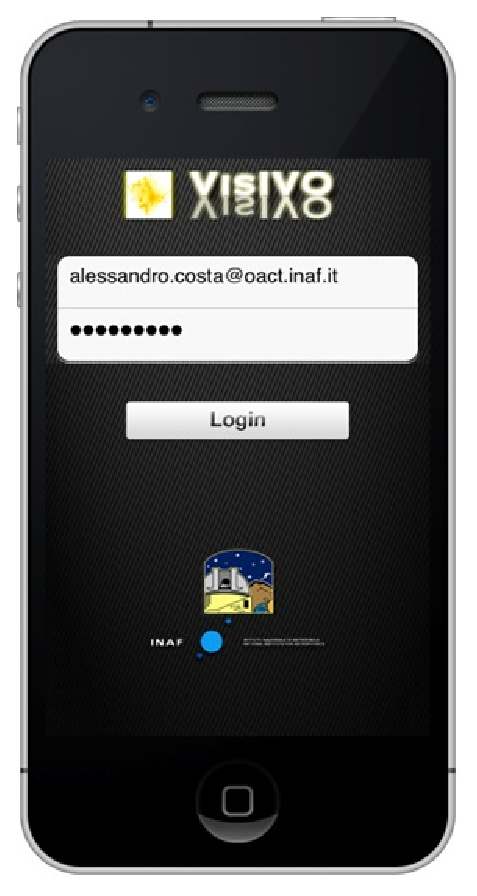
\includegraphics[width=0.2\textwidth]{O08_f3.eps}
    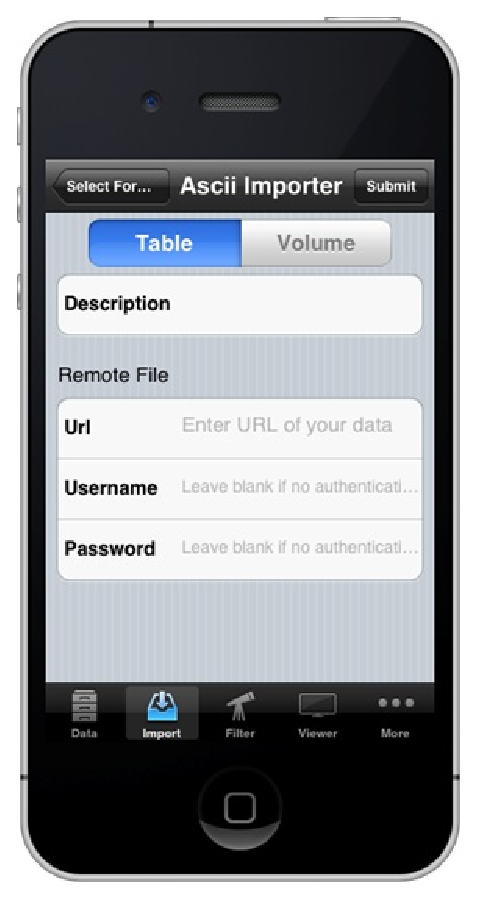
\includegraphics[width=0.2\textwidth]{O08_f4.eps}
    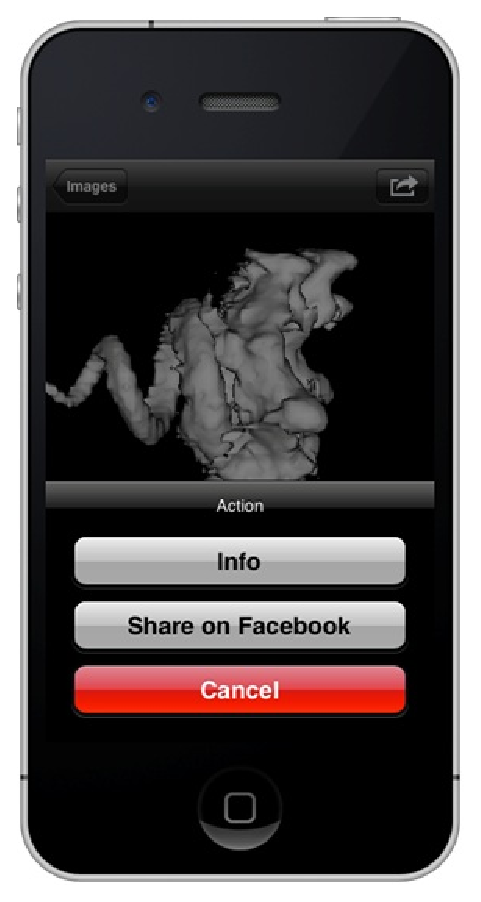
\includegraphics[width=0.2\textwidth]{O08_f5.eps}
    \caption{VisIVO Mobile Screenshots (from left to right) for Login, Remote Importing and Images Visualization.}
\label{fig:visivomobile}
\end{figure}

\section{VisIVO Mobile}
VisIVO Mobile  (see Figure \ref{fig:visivomobile}) is an application for iOS providing access to our scientific gateway by exploiting the widely used iPhone / iPad platforms. End users can login with the same credentials as with the gateway. The application allows encryption of passwords by using SHA1 cryptography and the results are base 64 encoded. Hashed passwords are sent to the server for the authentication phase. The classes that allow authentication can be re-used each time an iOS application is to be authenticated for a scientific gateway based on Liferay  and the software is released under GPL V.2. The mobile application is designed for intuitive browsing, importing and visualisation of user datasets.
\section{Summary}
Research in modern astrophysics is facing a data avalanche represented by exponential growth of datasets obtained through observations or numerical simulations. VisIVO Science Gateway is addressing this challenge by providing an interface for exploiting DCI resources in a transparent way and a rich set of visualization tools for handling large-scale datasets. This is realized in an environment for creating and sharing visualization workflows.  

\acknowledgements The research leading to these results has received funding from the European Union Seventh Framework Programme (FP7/2007-2013) under grant agreement no 283481 (SCI-BUS).

\bibliography{O08}

\end{document}
